\subsection*{Question 3.5}

From figure \ref{fig:q35hc} we see the hirarchical clustering, as
example we can take a closer look at the bottom two (the \emph{OVA})
as these are very close, which is indicated by the length of the lines
before the two are combined into the same cluster. As opposition to
this, we can look at the \emph{REN} cancer types being the three upper
ones. These are somewhat similar, but the lines are very long meaning
that they are not all that similar, but more similar to eachother than
to other cancer types. It is also interesting too look at the other
group of three \emph{REN} cancer types, these are much more similar
too eachother. There are some deviation from the \emph{pc}-plot, if it
followed it to the point we would expect to find \emph{MEL} and
\emph{NSC} in the same cluster in figure \ref{fig:q35hc}, but this is
not so. We also see that \emph{LEU} is not present in the figure,
which puzzles us a bit. But \emph{LEU} clusters nicely on it own,
meaning that it is mostly surrounded by its own types withing the
\emph{pc}-plot.

\begin{figure}[!htbp]
  \centering 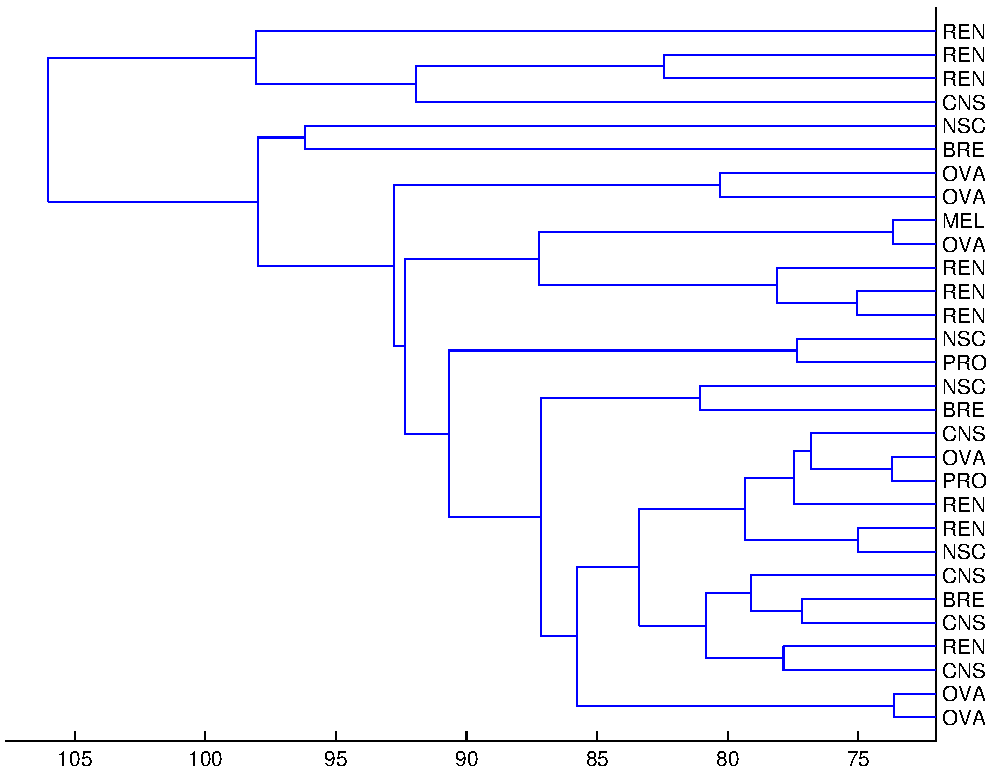
\includegraphics[width=0.95\textwidth]{./images/q35hc}
  \caption{Shows the hirarchical clustering}
  \label{fig:q35hc}
\end{figure}

\newpage

From figure \ref{fig:q35hm} we see the two-way hirarchical
clustering. From this we can see that the some of the same cancer
types produces the almost the same gene expression, looking at
\emph{LEU} and at the lower right corner, we see that the samples
$15$, $16$ and to some degree $14$ all has the same expression
level. And a similar pattern is shown over the rest of the heatmap. We
can see that the same cancer types tends to like clustered together
and quite similar gene expression profiles.

\begin{figure}[!htbp]
  \centering 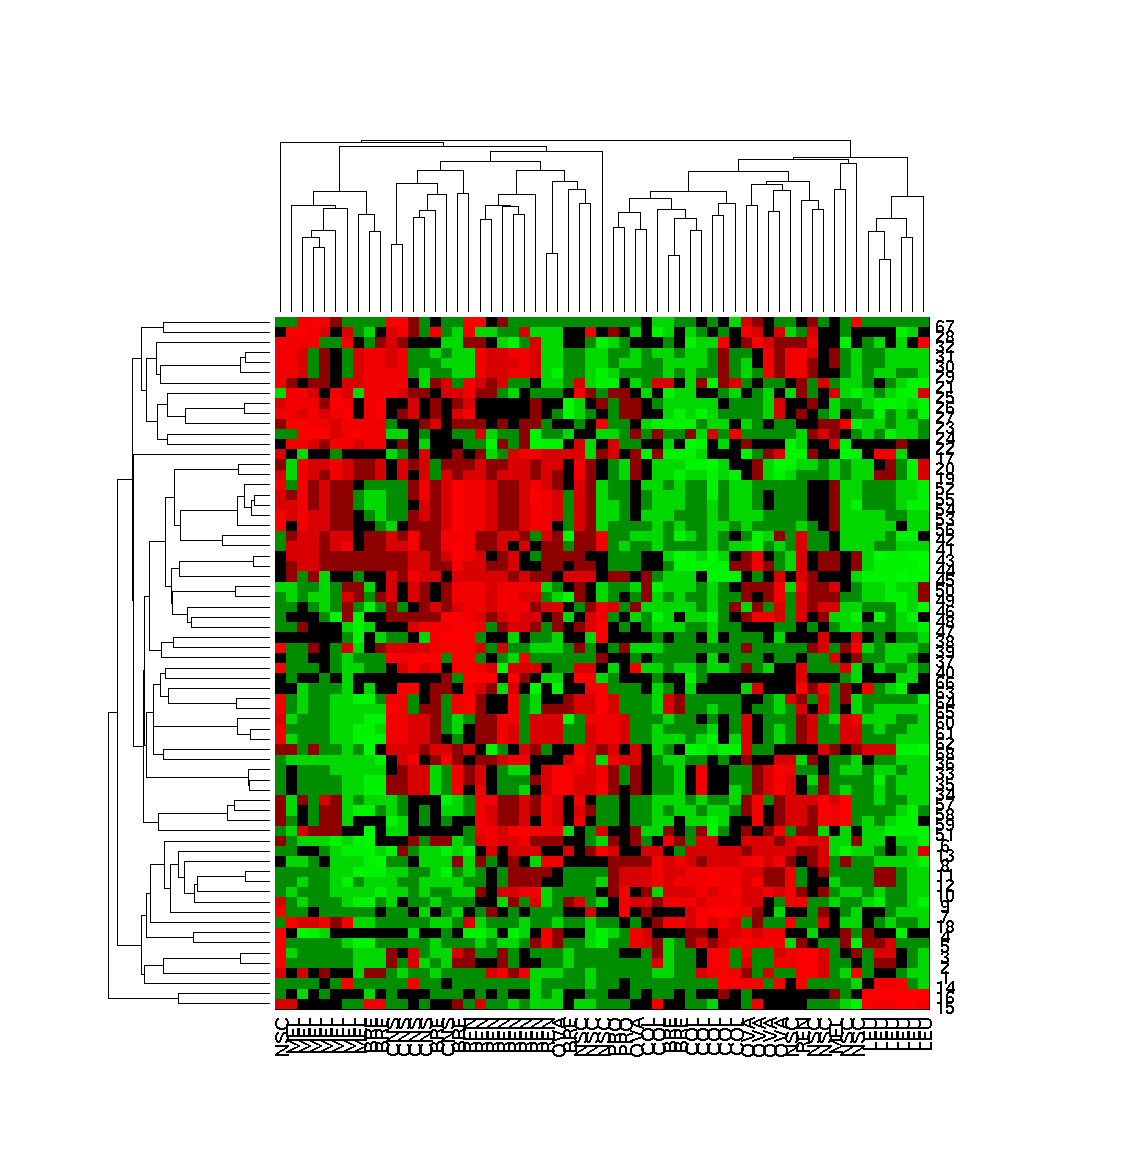
\includegraphics[width=0.95\textwidth]{./images/q35hm}
  \caption{Shows the heat map of the reduced sample set}
  \label{fig:q35hm}
\end{figure}
